\section{Broadcast}
\label{sec:prop-pres-case-studies:broadcast}
Broadcast is a system of fifteen processes communicating via three-party broadcast, i.e.\ three processes at a time synchronize simultaneously.
Figure~\ref{fig:prop-pres-case-studies:broadcast-network} shows two pairs of three such processes.
For each group of three processes, there is a synchronization rule that states that actions \action{a1}, \action{a2}, and \action{a3} synchronize.

\begin{figure}[hbt]
\centering
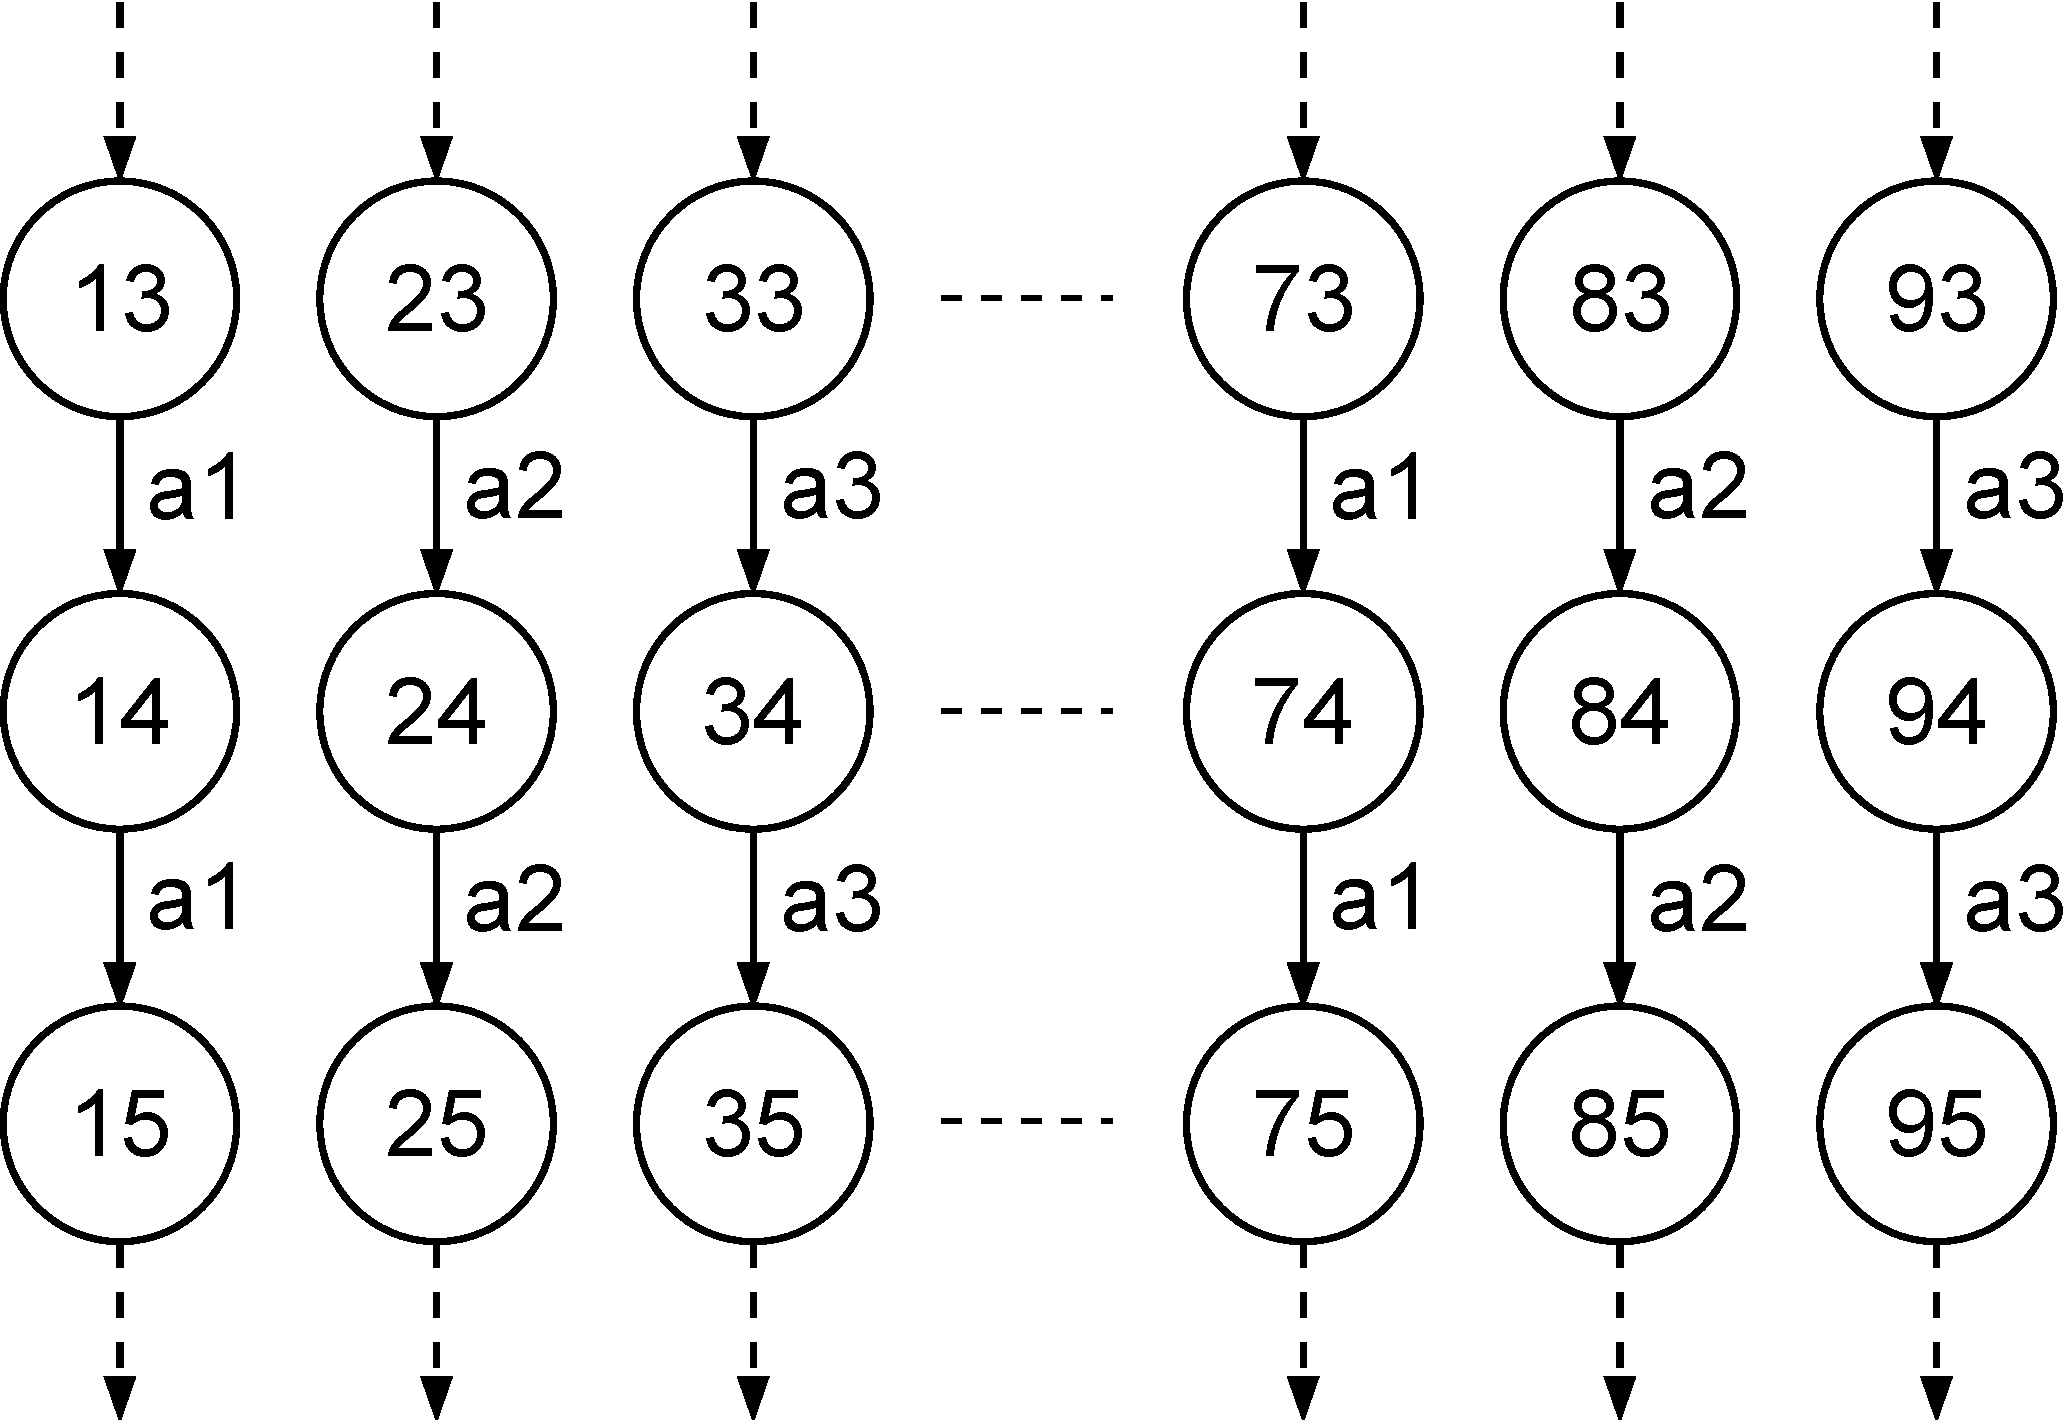
\includegraphics[scale=0.18]{prop-pres-case-studies/figs/broadcast-network}
\caption{Groups of three processes that communicate via broadcast}
\label{fig:prop-pres-case-studies:broadcast-network}
\end{figure}

Due to restrictions imposed by an implementation platform, a transformation that breaks this down into a series of two-party synchronization might be desired.
Three transformation rules that refine a model in this way are shown in Figure~\ref{fig:prop-pres-case-studies:faulty-broadcast-rules}.
After transformation, new synchronization rules are introduced that define that \action{a1'} and \action{a2'}, and  \action{a2''} and \action{a3'} synchronize.
This naive refinement does not preserve properties.

\begin{figure}[hbt]
\centering
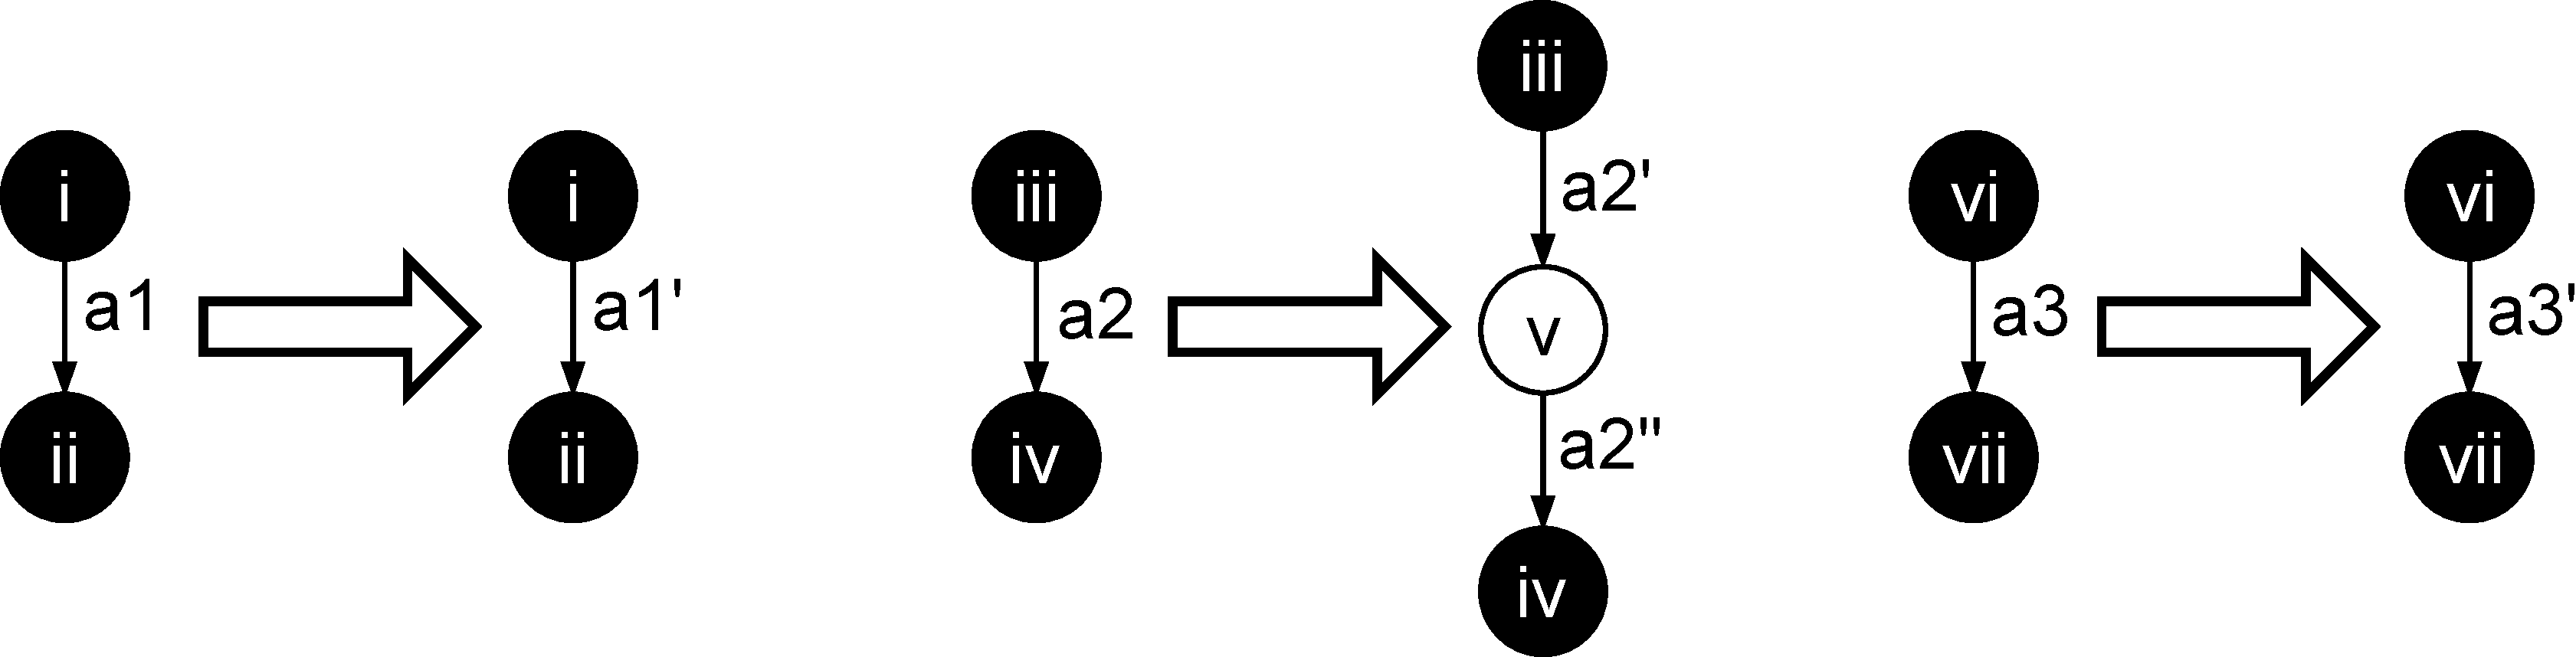
\includegraphics[scale=0.2]{prop-pres-case-studies/figs/faulty-broadcast-rules}
\caption{Transformation rules that replace a three-party broadcast by pairwise communication}
\label{fig:prop-pres-case-studies:faulty-broadcast-rules}
\end{figure}

Improved versions of these transformation rules are shown in Figure~\ref{fig:prop-pres-case-studies:broadcast-rules}.
Actions~\action{a2} and \action{a3} are replaced by \action{a2'} and \action{a3'}, respectively, to make the rule system terminating and confluent.
After transformation, new synchronization rules are introduced that define that
\begin{itemize*}
\item \action{m1a1} and \action{m2a1},
\item \action{c1a1} and \action{c2a1},
\item \action{a1a1} and \action{a2a1}, and
\item \action{a2'} and \action{a3'}
\end{itemize*}
synchronize.
The dashed $\tau$-transitions in Figure~\ref{fig:prop-pres-case-studies:broadcast-rules} indicate that this transformation is only property preserving if state~$i$ is matched on states that are diverging.

\begin{figure}[hbt]
\centering
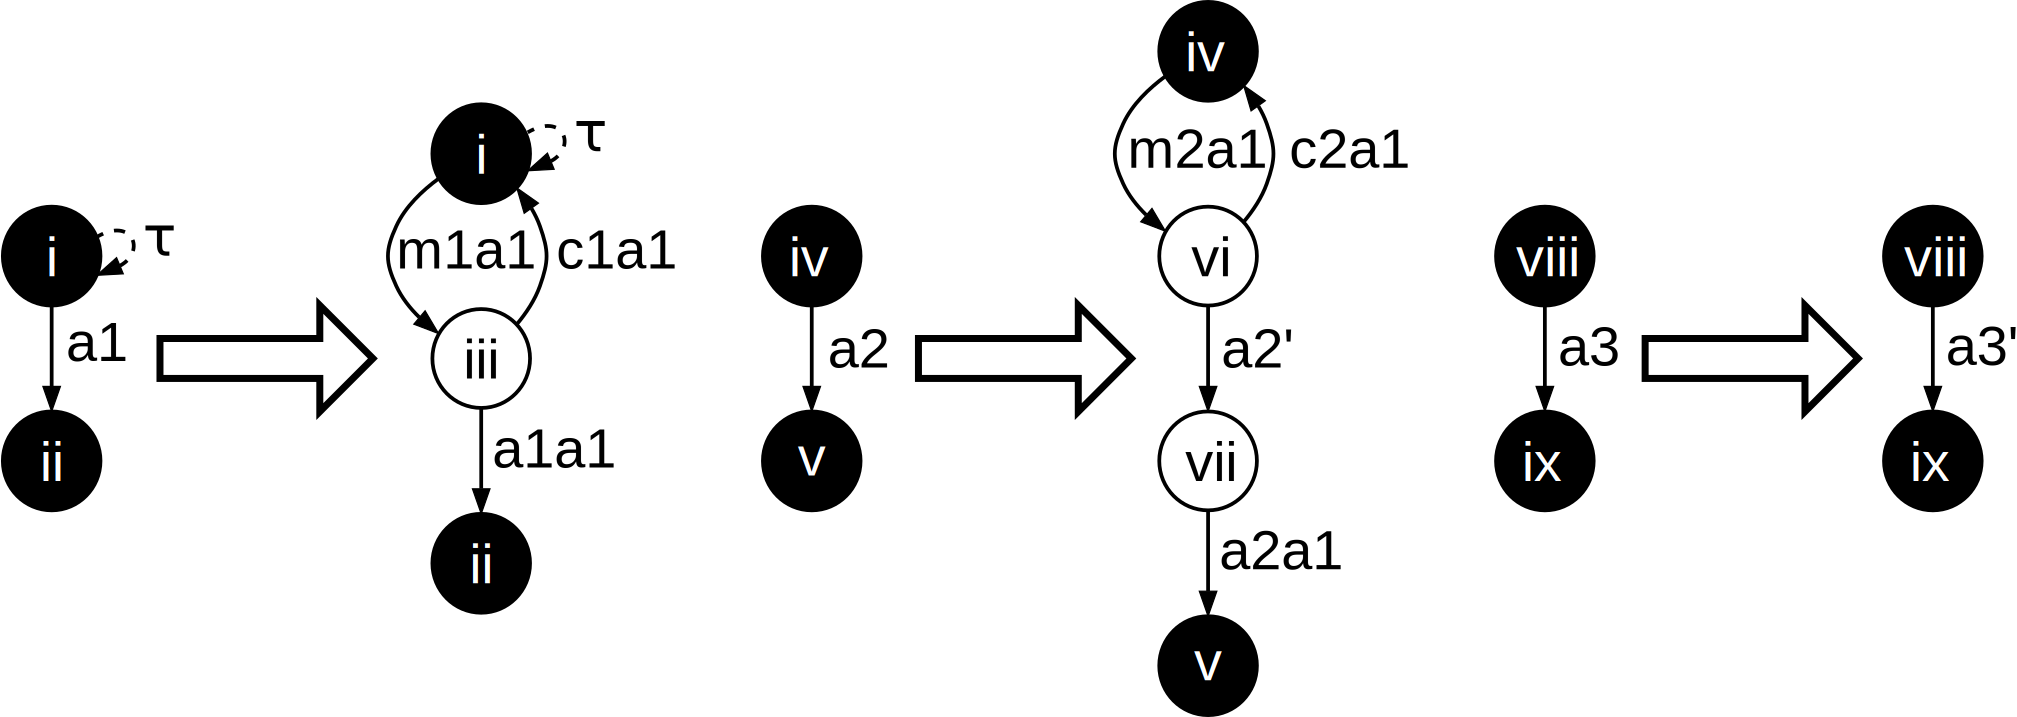
\includegraphics[scale=0.2]{prop-pres-case-studies/figs/broadcast-rules}
\caption{Three improved transformation rules that replace a three-party broadcast by pairwise communication}
\label{fig:prop-pres-case-studies:broadcast-rules}
\end{figure}

To check whether the transformation rules of Figure~\ref{fig:prop-pres-case-studies:broadcast-rules} preserve properties, a number of checks have to be performed.
Figure~\ref{fig:prop-pres-case-studies:broadcast-lhs} show some of the LTSs that are used for these checks.
The LTSs in Figure~\ref{fig:prop-pres-case-studies:broadcast-lhs} are created from the left-hand sides of the three transformation rules in Figure~\ref{fig:prop-pres-case-studies:broadcast-rules}.
The tools \EXPOPEN and \ltscompare of the \mCRLTwo toolkit cannot handle LTSs with multiple initial states.
To be able to use these tools to perform the checks, one initial state is added to each of the LTSs, as well as $\tau$-transitions to the original initial states.
Figure~\ref{fig:prop-pres-case-studies:broadcast-lhs} also show the $\kappa$-loops that are added to the original initial states.
Each of the checks determines whether a network consisting of a combination of LTSs created from the left-hand sides of transformation rules is divergence-sensitive branching bisimilar with the network consisting of the corresponding LTSs created from the right-hand sides, after hiding the appropriate actions in both networks.

\begin{figure}[hbt]
  \begin{minipage}[b]{4cm}
    \centering
    
\includegraphics[scale=0.2]{prop-pres-case-studies/figs/broadcast-rule1-lhs}
  \end{minipage}
  \hfill
  \begin{minipage}[b]{4cm}
    \centering
    
\includegraphics[scale=0.2]{prop-pres-case-studies/figs/broadcast-rule2-lhs}
  \end{minipage}
  \hfill
  \begin{minipage}[b]{4cm}
    \centering
    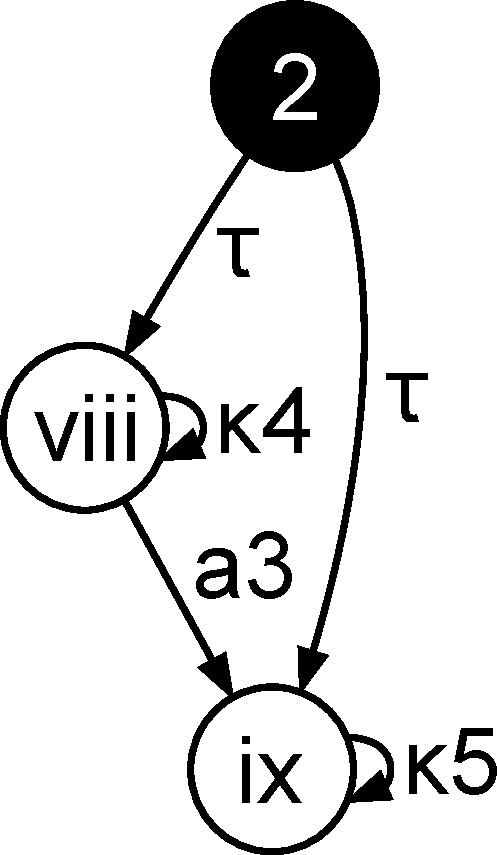
\includegraphics[scale=0.2]{prop-pres-case-studies/figs/broadcast-rule3-lhs}
  \end{minipage}
  \caption{Process LTSs of the left-hand sides of the transformation rules in Figure~\ref{fig:prop-pres-case-studies:broadcast-rules}}
  \label{fig:prop-pres-case-studies:broadcast-lhs}
\end{figure} 